\documentclass[../main.tex]{subfiles}
\begin{document}
\chapter{Lecture 9 - 06-04-2020}

$\hat{h}$  is ERM predictor
\\
$$
\ell_D\left(\hat{h}\right) \leq min \, \, \ell_D\left( h \right) + \sqrt[]{\frac{2}{m} \, \ln \, \frac{2 \, H}{\delta}} \qquad \textit{ with prob. at least $1-\delta$}
$$
\\
Now we do it with tree predictors\\
\section{Tree predictors}
$$
X  = \{ 0,1\}^d \longrightarrow \blue{Binary classification}
$$
$$
h : \{0, 1 \}^d \longrightarrow \blue{Binary classification H}1
$$
How big is this class? 
\\Take the size of codomain power the domain $\longrightarrow $ $|H| = 2^{2^d}$\\
Can we have a tree predictor that predict every H in this class?
\\
For every $ h : \{0,1\}^d$ $\longleftrightarrow$ $\{-1,1\} \quad \exists T$\\\\
We can \bred{build a tree } such that \quad $h_T = h$
\begin{figure}[h]
    \centering
    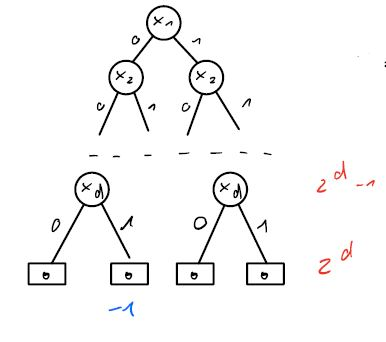
\includegraphics[width=0.6\linewidth]{../img/lez9-img1.JPG}
    \caption{Tree building}
    %\label{fig:}
\end{figure}\\
$ X = (0,0,1,...,1) \qquad h\left(x\right) = -1$ \\
$
\blue{$
x_1,x_2,x_3,...,x_d$}
$
\\\\
I can apply my analisys to this predictors
\\
If I run ERM on $H$ 
$$
\ell_D\left(\hat{h}\right) \, \leq \, min \, \ell_D \left(\hat{h}\right) + \sqrt[]{\frac{2}{m} \, 2^d  \, \ln 2 + \ln \frac{2}{\delta}} \qquad \longrightarrow \bred{$\ln|H|+\ln \frac{2}{\delta}$}
$$
No sense! What we find about training set that we need?
\\
Worst case of overfitting $m >> 2^D = |X|$ $\Rightarrow$ training sample larger
\\\\
\textbf{PROBLEM: }cannot learn from a class to big ( $H$ is too big)
\\
I can control $H$ just limiting the number of nodes.
\\\\
$H_N$ $\longrightarrow$  tree T with at most $N$ node, $N << 2^D$
\\
$|H_N| = \, ?$
\\
$$
|H_N| = \left( \textit{\# of trees with } \leq N \, nodes \right) 
\times
\left(  \textit{\# of test on interval nodes }  \right) 
\times
\left(  
\textit{ \# labels on leaves} 
\right) 
$$
$$
|H_N| = \red{\bigotimes} \, \times \, d^M \, \times 2^{N-M}
$$
$N$ of which $N-M$ are leaves
\begin{figure}[h]
    \centering
    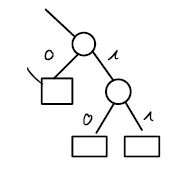
\includegraphics[width=0.6\linewidth]{../img/lez9-img2.JPG}
    \caption{Tree with at most N node}
    %\label{fig:}
\end{figure}\\
$$\red{\bigotimes}
\textit{\# of binary trees with N  nodes, called \bred{Catalan Number}}
$$
\subsection{Catalan Number}
*We are using a binomial *
$$
\frac{1}{N} \binom{2 \, N -2}{N-1} \quad \leq \quad \frac{1}{N} \, \left(e \, \frac{\left(2\, N -2 \right)}{N-1} \right)^{N-1} = \frac{1}{N} \, \left( 2 \, e \right)^{N-1}
$$
$$
\binom{N}{K} \quad \leq \quad \left( \frac{e\, n}{k}\right)^k \qquad \textit{ from Stirling approximation}
$$
Counting the number of tree structure: a binary tree with exactly N nodes.
Catalan counts this number. $\longrightarrow$ \blue{but we need a quantity to interpret easily}. So we compute it in another way.
\\
Now we can rearrange everything.
\\
$$ | H _N | 
\quad \leq \quad  \blue{ $
\frac{1}{N}$} \, \left( 2 \, e \right)^{N-1} \, H^M \, \bred{$2^{N-M} $}
\quad  \leq \quad 
\left( 2 \, e \, d \right)^N
$$
\qquad \qquad \qquad \qquad \qquad \qquad \qquad 
\bred{$d \geq 2$} \qquad \bred{$\leq \, d^{N-M}$ }\\
where \blue{we ignore $
\frac{1}{N}$ since we are going to use the $\log$}
\\\\
ERM on $H_N \quad \hat{h} \quad $ 
$$\ell_D \left(\hat{h}\right) \, \leq \, \min_{\mathbf{h \, \in\, H_N}} \, \ell_D \left( h \right) + \sqrt[]{\frac{2}{m} \,  \left( \bred{$   N \cdot \left( 1+ \ln \left(2 \cdot d \right) \right)$} + \ln \frac{2}{\delta} \right) }
$$
\\
were  \bred{$   N \cdot \left( 1+ \ln \left(2 \cdot d \right) \right)$}  \quad $= \quad  \ln \left( H_N \right) 
$\\\\
In order to not overfit $ m >> N \cdot \ln d
$\\
$N \cdot \ln d << 2^d$ for reasonable value of $N$
\\
We grow the tree and a some point we stop.
$$
\ell_D\left(h\right) \, \leq \, \hat{\ell}_S \left(h\right) + \varepsilon 
\qquad \forall h \in H_N \qquad \textit{with probability at least $1-\delta$}
$$
\\
\bred{remove $N$ in $H_N$ and include $h$ on $\varepsilon$}
\\
we remove the $N$ index in $H_N$ adding $h$ on $\varepsilon$

$$
\ell_D \left(h\right) \, \leq \, \hat{\ell}_S \left(h\right) + \varepsilon_{\red{h}} \qquad \forall h \in H_{\not{\red{N}}}
$$
$$
W : H \longrightarrow \left[ 0,1 \right] \qquad \sum_{h\in H}{} w\left(h\right) \leq 1
$$
\\
\blue{How to use this to control over risk?}
$$
\barra{P} \left( \exists h \in H \, : \, | \, \hat{\ell}_S \left(h \right) - \ell_D \left( h \right) \, | \, > \varepsilon_h \right) \quad \leq
$$
\bred{where $\hat{\ell}_S$ is the prob my training set cases is true}
$$
\leq \, 
\sum_{h \in H}{} 
\barra{P} \left( \, | \, \hat{\ell}_S 
\left(h \right) 
- 
\ell_D 
\left( h \right) 
\, | \, 
> \varepsilon_h \right) \, \leq \, \sum_{h \in H}{} 2 \, e^{-2 \, m \, \varepsilon \, h^2 } \, \leq \, $$
$$
\leq \, \delta \qquad \longrightarrow \textit{since $w(h)$ sum to $1$ $ \left( \, \sum_{h \in H} \, \right)  $}
$$
I want to choose \bred{$ \quad 2 \, e^{-2 \, m \, \varepsilon \, h^2 } \, =\, \delta \, w(h)$}
\\
$$
2 \, e^{-2 \, m \, \varepsilon \, h^2 } \, =\, \delta \, w(h) \qquad \Leftrightarrow \qquad \textit{--- MANCA PARTEEEE --- }
$$\\
therefore:
$$
\ell_D \left(h \right) \leq 
\hat{\ell}_S \left(h\right) + 
\sqrt[]{\frac{1}{2 \, m} \cdot \left( \ln \frac{1}{w(h)} + ln \frac{2}{\delta} \right) } \quad \textit{w. p. at least $1-\delta$ \quad $\forall h \in H$} 
$$
\\
Now, instead of using ERM we use
$$
\hat{h} = arg\min_{h \in H} \left(\hat{\ell}_S\left( h \right) 
+ 
\sqrt[]{ \frac{1}{2 \, m} \cdot \left( \ln \frac{1}{w(h)} + ln \frac{2}{\delta} \right) }
\right)
$$
\bred{where $\sqrt[]{...}$ term is the penalisation term}
\\\\
Since our class is very large we add this part in order to avoid overfitting. \\
Instead of minimising training error alone i minimise training error +
penalisation error.\\\\
In order to pick w(h) we are going to use \bred{coding theory}\\
The idea is I have my trees and i want to encode all tree predictors in H using
strings of bits.
\\\\
$\sigma : H $ $\longrightarrow $ $\{ 0,1 \}^* \qquad \bred{coding function for trees}
$
\\
$\forall \, h, h' \in H$ \qquad $\sigma(h)$ not a prefix of $\sigma(h') 
$\\
$h \neq h'$ \qquad \qquad where $\sigma(h)$ and $\sigma(h')$ are \bred{string of bits}
\\\\
$\sigma$ is called \blue{istantaneous coding function}
\\
Istantaneous coding function has a property called \bred{kraft inequality}
$$
\sum_{h\in H}{} 2^{-|\, \sigma\left(h\right)\, |} \leq 1 \qquad w(h) = 2^{-|\,\sigma(h)\,|}
$$
\\
I can design $\sigma : H \longrightarrow \{0,1\}^* \quad  istantaneous \ |\,\sigma(h)\,|$\\

$
\ln |H_N| = O\left(N \cdot \ln d\right) 
$\\
\bred{number of bits i need \quad $=$ \quad number of node in $h$}
\\\\
Even if i insist in istantaneous i do not lose ... -- MANCA PARTE --
\\
$$
| \, \sigma (h) \, | = O \left( N \cdot \ln d\right)
$$\\
Using this $\sigma$ and $w(h) = 2 ^{-|\, \sigma(h)\,|}
$
$$
\ell_D\left(h\right) \, \leq \, \hat{\ell}_S \left( h \right) + \sqrt[]{\frac{1}{2 \, m} \cdot \left( \red{c} \cdot N \cdot \ln d + \ln \frac{2}{\delta} \right) } \qquad \textit{w. p. at least $1-\delta$}
$$
where \red{$c$} is a constant
\\
$$
\hat{h} = arg\min_{h\in H} \left( \hat{\ell}_S \left( h \right) + \sqrt[]{\frac{1}{2 \, m} \cdot \left( \red{c} \cdot N \cdot \ln d + \ln \frac{2}{\delta} \right) } \, \right)
$$
where \bred{$m >> N \cdot h \cdot \ln d$}
\\
If training set size is very small then you should not run this algorithm.
\begin{figure}[h]
    \centering
    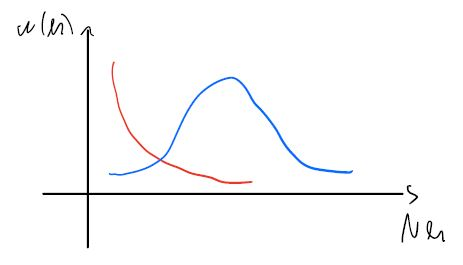
\includegraphics[width=0.6\linewidth]{../img/lez9-img3.JPG}
    \caption{Algorithm for tree predictors}
    %\label{fig:}
\end{figure}\\
This blue curve is an alternative example. We can use Information criterion.\\\\
As I increase the number of nodes, $N_h$ decrease so fast. You should take a
smaller tree because it gives you a better bound. It’s a principle known as
Occam Razor ( if I have two tree with the same error, if one is smaller than the
other than i should pick this one).
\\\\
Having $N^*$
\end{document}